\begin{center}
    \centering
    \begin{tabular}{|c|c|c|c|}
    \hline
        $n_\text{glass}$ & $\frac{\partial n_\text{glass}}{\partial t}$ & $\frac{\partial n_\text{glass}}{\partial d}$ & Error of $n_\text{glass}$ \\ \hline
        1.39 & 0.34 & -0.08 & 0.08 \\ \hline
        \multicolumn{4}{|c|}{$\bm{n_\textbf{glass}: 1.39\pm0.08}$}\\\hline
    \end{tabular}
    \vspace{3mm}
    \\ Table 5: $n_\text{glass}$ Final Value by Pfund's Method\\
    \vspace{5mm}
    \centering
    \begin{tabular}{|c|c|c|c|c|c|}
    \hline
        $n_\text{liquid}$ & $\frac{\partial n_\text{liquid}}{\partial t}$ & $\frac{\partial n_\text{liquid}}{\partial d}$ & $\frac{\partial n_\text{liquid}}{\partial n_{\text{glass}}}$ & Error of $n_\text{glass}$ & Error of $n_\text{liquid}$ \\ \hline
        1.29 & -0.09 & 0.009 & 0.93 & 0.08 & 0.26 \\ \hline
        \multicolumn{6}{|c|}{$\bm{n_\textbf{liquid}: 1.29\pm0.26}$}\\\hline
    \end{tabular} 
    \vspace{3mm}
    \\ Table 6: $n_\text{liquid}$ Final Value by Pfund's Method\\
    \vspace{5mm} 
    \centering
    \begin{tabular}{|c|c|c|c|}
    \hline
        $n_\text{liquid}$ & $\frac{\partial n_\text{liquid}}{\partial \theta_1}$ & $\frac{\partial n_\text{liquid}}{\partial \theta_2}$  & Error of $n_\text{liquid}$ \\ \hline
        1.62 & 1.88 & -3.82 & 0.04  \\ \hline
        \multicolumn{4}{|c|}{$\bm{n_\textbf{liquid}: 1.62\pm0.04}$}\\\hline
    \end{tabular} 
    \vspace{3mm}
    \\ Table 7: $n_\text{liquid}$ Final Value by Snell's Law\\
    \vspace{5mm}
    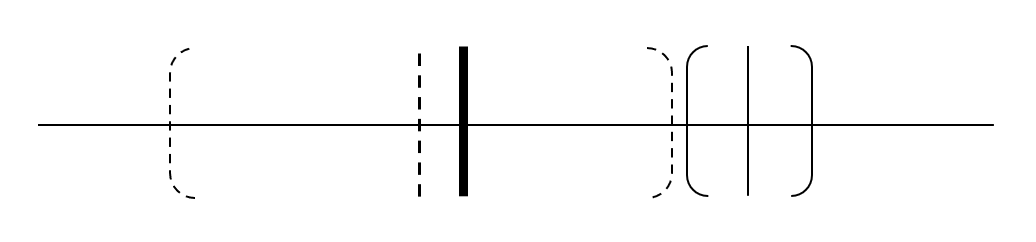
\includegraphics[scale=0.5]{number line.png}\\
    Dashed = Method 1 (Pfund's Method)\\
    Solid = Method 2 (Snell's Law)\\
    Bold = Accepted Value \\
    Figure 1: Number Line Indicating Error Bounds and Accepted Values   
\end{center}
Using Figure 1, we can see that while the index of refraction calculated via Pfund's Method had a greater error, it was closer to the accepted value of the index of refraction of water, which is 1.33. The accepted index of refraction lies within the error bounds of the Pfund's Method calculation. Snell's method provided an index of refraction of $1.62\pm0.04$ which does not agree with the accepted value. This can mainly be attributed to human error in measuring the incident and refracted angles. When measuring our angles, we misread our protractor as having increments at every $1\degree$, as opposed to every $0.5\degree$. This provided us with an instrumental error of $0.5\degree$, as opposed to $0.25\degree$.
\\\indent The error introduced in Pfund's Method stems from multiple areas. Firstly, the petri dish may not have had a uniform thickness, providing different thickness readings on the micrometer. Then, the laser may not have been pointed perfectly vertically. Pfund's method relies on the laser making an angle of $\frac{\pi}{2}$ with the horizontal. Lastly, error is introduced in measuring each of the rings. The method of measuring required eyeballing where the ring lined up on the polar grid and then measuring the polar grid on a separate piece of paper. Measurements were taken using a pair of vernier calipers, which have pointed ends where the measurements are taken. These tended to make indentations in the polar grid paper which the calipers would slide into when taking other measurements.\\
\indent The second method using Snell's Law had less error associated with the final index of refraction relative to the value found by Pfund's Method. The calculated index of refraction is $1.62\pm0.04$. While tracing the petri dish onto our surface, the polar grid on the bottom of the dish caused us to trace a larger circle than the diameter of the petri dish. Then, when placing the pins along the path of the laser, the laser may have been nudged out of position. This would affect the accuracy of our measured angles. The center of the circle may also have been misplaced, as it is found using the perpendicular bisectors of two cords. These perpendicular bisectors may not have been exactly perpendicular. This would affect the measurements taken for our angles, and in turn affect our index of refraction.